\documentclass{article}

% NeurIPS 2025 style (vendored in neurips/neurips_2025.sty), preprint mode:
% these are self-study reports, not conference submissions.
\PassOptionsToPackage{numbers,sort&compress}{natbib}
\usepackage[preprint]{neurips/neurips_2025}

\usepackage[T1]{fontenc}
\usepackage{amsmath,amssymb}
\usepackage{booktabs}
\usepackage{graphicx}
\usepackage{array}
\usepackage[table]{xcolor}
\usepackage{tikz}
\usetikzlibrary{positioning,arrows.meta}
\usepackage[colorlinks=true,linkcolor=blue,urlcolor=blue,citecolor=blue]{hyperref}

% Okabe-Ito-derived palette for Part II status figures and the compatibility
% matrix: status is always paired with a written label, never carried by
% color alone.
\definecolor{nativecol}{HTML}{0072B2}
\definecolor{genericcol}{HTML}{009E73}
\definecolor{partcol}{HTML}{E69F00}
\definecolor{unattcol}{HTML}{D55E00}

\newcolumntype{L}[1]{>{\raggedright\arraybackslash}p{#1}}
% neurips_2025 preprint mode does not update \textwidth (see the geometry
% \newgeometry caveat in neurips_2025.sty), so column widths are literal.
\newlength{\dimcol}\setlength{\dimcol}{3.7cm}
\newlength{\lblcol}\setlength{\lblcol}{1.9cm}

\newcommand{\codex}[0]{Codex}
\newcommand{\occ}[0]{OpenCode}
\newcommand{\ccc}[0]{Claude Code}

\title{Claude Code, Codex, and OpenCode at the Source Level:\\
Harness Architecture and Open-Source Model Support\\
{\large A Static Source-Trace Study at Pinned Commits}}
\author{self-study-with-ai}
\date{\today}

\begin{document}
\maketitle

\begin{abstract}
A coding agent is a language model inside a loop: the model proposes,
tools act on a repository, observations return, and the surrounding
software, the harness, decides whether to continue. This study examines
the three production harnesses \ccc{}, \codex{}, and \occ{} with two
questions. Part I asks how they are built: because the \ccc{} core is
closed source, we pin all three repositories and restrict the study to
static source traces and official documentation snapshots, with 300
anchors re-verifying against the pinned commits. Part II asks what
happens when the model on the other end is open source: through which
surface each agent reaches Ollama, LM Studio, and generic
OpenAI-compatible servers, and what degrades there. The three systems
implement the same abstract loop and the same anti-loop instinct, then
diverge structurally: \codex{} is a typed state machine with an OS
sandbox and a rule engine, \occ{} a persistence-driven loop with
permissive defaults and per-step revert, \ccc{} a documented contract
over a closed core. Open-model support divides just as cleanly, and the
dividing variable is the wire protocol each harness commits to:
\codex{} ships native Responses-API providers for two local servers at
the cost of its patch tool, \occ{} accepts anything
chat-completions-shaped while its accounting defaults silently misbehave
around zero limits, and \ccc{} documents no open-model surface at all.
The architecture findings explain the compatibility findings: provider
plumbing is where each harness's engineering culture shows through
first. All findings are bounded to the pinned commits (\path{af70018},
\path{d545d8f}, \path{c3d2e35}) and the documentation snapshots of
2026-08-20.
\end{abstract}

\section{Introduction}

A coding agent is a loop: the model proposes, tools act on a repository,
observations return, and the harness decides whether to continue. The
model supplies only the middle step: it cannot itself read files, execute
commands, or remember what happened last iteration. The harness, all the
software around the model, supplies everything else: the continuation
condition, the tool surface the model sees, the context budget, the
permission system, and the extension point where users bend the agent to
their workflow. This decomposition has research pedigree. ReAct interleaves reasoning traces
with environment actions and showed the combination beats either alone on
question answering and interactive tasks~\citep{yao2023react}. Toolformer
trained a model to emit, execute, and resume around API calls,
establishing the interrupt-execute-resume protocol that every agent harness
now re-implements in engineering form~\citep{schick2023toolformer}. SWE-agent
demonstrated that the interface itself is a first-order factor: an
agent-tailored computer interface with a guarded edit command and lint
gating raised SWE-bench Lite resolution from 11.0\% (shell-only) to 18.0\%
with GPT-4 Turbo, without changing the model~\citep{yang2024sweagent}.

What the literature leaves open is how this interface layer is built in
the shipping products that practitioners use. We study three of
them, \ccc{}, \codex{}, and \occ{}, at pinned source versions, and ask
two primary questions. \textbf{Part I} asks how the harnesses are built:
what components make up a coding-agent harness, where the three systems
genuinely differ, how each trades capability against safety, and what
the closed \ccc{} core reveals through documentation, its plugin
surface, and third-party teardowns. \textbf{Part II} asks what the same
harnesses do with open-source models: whether each can reach a local or
generic open-model server, through which integration surface (native
provider code, generic OpenAI-compatible endpoint, or documentation
only), and where support degrades, because a coding agent that can run
against a local model is a platform in a way that one bound to a closed
model list is not.

The answer, in one sentence per part. Part I: the abstraction has
converged, an eight-dimension harness with one shared loop, but the
engineering cultures have not, and the systems differ in where they
place the trust boundary, how durable they make their state, and how
much they hide. Part II: compatibility is decided by the wire protocol
each agent commits to, and each commitment has a matching price. The two
readings reinforce each other: provider plumbing is the configuration
dimension of Part I under stress, and each system's open-model behavior
is exactly what Part I's architecture predicts
(Section~\ref{sec:synthesis}).

\paragraph{Systems under study.} \codex{} is OpenAI's open-source coding
agent (Apache-2.0), a Rust core dispatched from one binary to a terminal
UI, a headless exec mode, and app-facing
servers~\citep{codexRepo}. \occ{} is the open-source
TypeScript coding agent of the \texttt{anomalyco/opencode} project (MIT),
studied at the \texttt{dev} branch of its rewrite rather than a numbered
release; it pairs a terminal UI with a local HTTP server and editor-facing
protocols~\citep{opencodeRepo}. \ccc{} is Anthropic's
coding agent: its core is closed source, distributed behind CLI, IDE, and
desktop surfaces, and its public repository carries only the plugin and
example surface~\citep{claudeCodeSurface,claudeCodePermissionsDocs}.

The \ccc{} core is closed source, and its pinned public checkout contains no
harness code~\citep{claudeCodeSurface}. We therefore treat documentation
snapshots as the evidence tier for that system, hold third-party teardowns
to hedged context only, and mark closed-core internals as boundaries rather
than findings. Contributions at the supported scope:

\begin{itemize}
  \item an eight-dimension decomposition of a coding-agent harness, grounded
  in three pinned implementations and the framing literature
  (Section~\ref{sec:components});
  \item four pre-registered static-trace extractions, turn loops, tool
  surfaces, safety policies, and compaction parameters, whose anchors all
  re-verify at the pinned commits (Section~\ref{sec:methods},
  Sections~\ref{sec:turnloop} to~\ref{sec:compaction});
  \item a dimension-by-dimension comparison that separates genuine
  structural differences from naming differences
  (Sections~\ref{sec:extensibility} to~\ref{sec:state});
  \item an open-source model compatibility trace covering three integration
  surfaces per agent plus the server-side contract of three reference
  servers, with every cell a code path, a documentation contract, or a
  labeled gap (Sections~\ref{sec:servers} to~\ref{sec:matrix}).
\end{itemize}

\section{Background}
\label{sec:background}

\paragraph{The abstract loop.} ReAct frames agency as an interleave of
thoughts, actions, and observations, and measured both its gains and its
failure modes: grounded search cut hallucinated failures from 56\% (chain
of thought) to 0\% of failures on HotpotQA, at the cost of a repetitive
failure pattern in which the model re-generates its previous thoughts and
actions~\citep{yao2023react}. Harness designers inherit both sides: a
continuation condition, and a defense against loops.

\paragraph{Tool calling as protocol.} Toolformer learns when to call a tool,
with what arguments, and how to fold results back into prediction, and
restricts decoding to at most one API call per input explicitly to prevent
runaway tool loops~\citep{schick2023toolformer}. The same concern appears in
all three harnesses as explicit machinery (Section~\ref{sec:turnloop}).

\paragraph{The agent-computer interface.} SWE-agent ablated interface
choices on SWE-bench Lite and found each one measurable: removing the edit
command dropped resolution by 7.7 points, disabling linting dropped it by
3.0 points, and an iterative search interface performed worse than no added
search tools at all~\citep{yang2024sweagent}. Editing is where agents spend
their failures: 51.7\% of instances had at least one failed edit, and the
probability of eventual edit success dropped from 90.5\% to 57.2\% after a
single failure~\citep{yang2024sweagent}. Guardrails trade flexibility for
recovery, a tradeoff our three systems resolve differently
(Sections~\ref{sec:tools},~\ref{sec:safety}).

\section{Methods and Sources}
\label{sec:methods}

\paragraph{Design.} Descriptive static source-trace study. The units of
analysis are literal code constructs at pinned commits and quoted
documentation text at pinned snapshots. There is no behavioral measurement:
no agent CLI was invoked, no live API was called, no server was started,
and no code from the pinned repositories was executed. The pinned checkouts
were treated as read-only untrusted data.

\paragraph{Pins and sources.} Three local checkouts were pinned on
2026-08-19 and re-pinned on 2026-08-20, confirming the same commits:
\path{af700180808cce2ce28a31aad0fbad4dc58b857a} (\codex{},
Apache-2.0), \path{d545d8fba57283528db69281f59c803c646eb7e9} (\occ{}, MIT,
\texttt{dev} branch), and \path{c3d2e35e554060b5a20ee6b28140fbdbd4eb0048}
(\ccc{})~\citep{codexRepo,opencodeRepo,claudeCodeSurface}. Official
documentation snapshots were fetched 2026-08-20; documentation sites are
not version-pinned and can drift, so documentation claims cite the snapshot
rather than a commit~\citep{claudeCodeHooksDocs,claudeCodeSubagentsDocs,%
claudeCodePluginsDocs,claudeCodeMcpDocs,claudeCodeMemoryDocs,%
claudeCodePermissionsDocs,claudeCodeSandboxingDocs,codexSandboxingDocs,%
opencodeDocs,codexDocsRepo,claudeCodeModelDocs,claudeCodeBedrockDocs}.
Evidence tiers: pinned code (primary for \codex{} and \occ{}), pinned
plugin/example surface plus documentation snapshots (the only tier
available for the \ccc{} core), framing preprints (background), and
third-party teardowns, \texttt{tier: blog}, admissible only for hedged
contextual statements~\citep{minusXTeardown,agiflowInternals,%
tenguDecoded,claudeCodeRouterContext}.

\paragraph{Part I trace experiments.} Four experiments were frozen in a plan
before any full extraction (EXP-PLAN-2026-08-19-v1): E1 turns loops, E2
tool surfaces, E3 safety policies, E4 compaction parameters. Each produced
markdown and JSON artifacts in which every stated value carries a
\path{file:line} or snapshot-line anchor, plus a validation script that
re-checks every anchor against the pinned sources. Results: 59/59 anchor
checks for E1, 131/131 for E2, 75/75 for E3, 35/35 for E4
(300 total); all three HEADs matched the pins at every validation. The
validation runs are smoke-test plumbing, not scientific evidence; the
extraction artifacts carry the findings. Twelve claims advanced to
ANALYZED with supported evidential status (\texttt{CLM-E1-1a} through
\texttt{CLM-E4-3a} in the study's claim ledger, each superseding its
EXECUTED counterpart; after review, \texttt{CLM-E2-1a} was itself
superseded by \texttt{CLM-E2-1b} correcting a registration count from 33
to 32). The claim ledger lived in the Part I study's dossier and is
preserved in its git history.

\paragraph{Part II traces.} Provider plumbing was traced in the same pinned
trees: the dedicated \codex{} Ollama and LM Studio crates, and \occ{}'s
provider module; \ccc{}'s loader is closed, so its column is filled from
documentation snapshots (model configuration and Amazon
Bedrock)~\citep{claudeCodeModelDocs,claudeCodeBedrockDocs}. The
server-side contract came from the reference servers' own documentation:
the 2024 Ollama OpenAI-compatibility post~\citep{ollamaCompatDocs}, LM
Studio's developer docs snapshotted via its public docs repository because
the live site was unreachable from the study
environment~\citep{lmstudioApiDocs}, and the llama.cpp server README at
master~\citep{llamaCppServerDocs}. Part II was scoped as a briefing:
extraction was anchored but not pre-registered as an experiment plan; its
12 notes (3 codebase, 8 documentation, 1 context) carry its evidence.
The Part I extractions oriented Part II but were never cited for it: every
Part II claim carries its own anchor.

\paragraph{Closed-core protocol.} The \ccc{} column is filled exclusively
from documentation quotes and the pinned plugin/example surface in both
parts. Where no pinned source states a value, the text says so explicitly
and the gap is listed in Section~\ref{sec:limitations}. Blog-tier teardowns
and community routers never fill a comparison cell on
their own~\citep{claudeCodeSurface,agiflowInternals,claudeCodeRouterContext}.

\part{Harness architecture}

\section{Findings}
\label{sec:findings}

\paragraph{How to read what follows.} Each subsection answers one design
question: what does a harness have to decide here, and how did each
system decide it? The tables carry the exact values with their anchors,
and are safe to skim; the prose interprets what each value means as a
design choice. Where a system's answer is unknown (the \ccc{} core is
closed), the cell says \emph{undisclosed} and the limit is restated in
Section~\ref{sec:limitations}.

\subsection{What makes a coding-agent harness}
\label{sec:components}

Cross-system, the harness decomposes into eight machinery dimensions, each
independently implemented by all three systems: the turn loop; the tool
surface and its file-edit protocol; context assembly and compaction;
persistent memory files; permission and sandbox policy; extensibility
(hooks, plugins, skills, subagents, MCP servers); configuration and model
provider plumbing; and session state with durable storage and user-facing
transports. The decomposition is the Part I contribution: it
reduces ``what is inside one of these products'' to eight questions that
every implementation must have an answer to (Figure~\ref{fig:anatomy}).
Table~\ref{tab:summary} summarizes the matrix; the details follow per
dimension.

\begin{figure}[t]
\centering
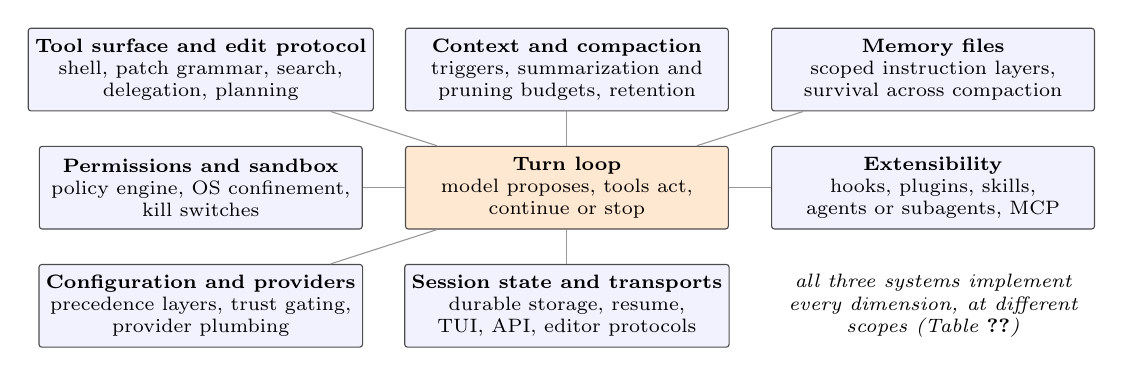
\begin{tikzpicture}[font=\scriptsize,
  box/.style={draw=black!70, rounded corners=1pt, align=center,
    minimum width=4.1cm, minimum height=1.05cm, inner sep=2.5pt,
    fill=blue!5, text=black},
  loop/.style={box, fill=orange!18},
  conn/.style={draw=black!40, line width=0.4pt}]
\node[loop] (loop) at (0,0) {\textbf{Turn loop}\\ model proposes, tools act,\\ continue or stop};
\node[box] (tools) at (-4.65, 1.5) {\textbf{Tool surface and edit protocol}\\ shell, patch grammar, search,\\ delegation, planning};
\node[box] (ctx)   at ( 0.0, 1.5) {\textbf{Context and compaction}\\ triggers, summarization and\\ pruning budgets, retention};
\node[box] (mem)   at ( 4.65, 1.5) {\textbf{Memory files}\\ scoped instruction layers,\\ survival across compaction};
\node[box] (perm)  at (-4.65, 0) {\textbf{Permissions and sandbox}\\ policy engine, OS confinement,\\ kill switches};
\node[box] (ext)   at ( 4.65, 0) {\textbf{Extensibility}\\ hooks, plugins, skills,\\ agents or subagents, MCP};
\node[box] (cfg)   at (-4.65,-1.5) {\textbf{Configuration and providers}\\ precedence layers, trust gating,\\ provider plumbing};
\node[box] (state) at ( 0.0,-1.5) {\textbf{Session state and transports}\\ durable storage, resume,\\ TUI, API, editor protocols};
\node[align=center, font=\scriptsize\itshape] at (4.65,-1.5)
  {all three systems implement\\ every dimension, at different\\ scopes (Table~\ref{tab:summary})};
\foreach \n in {tools,ctx,mem,perm,ext,cfg,state}
  \draw[conn] (loop) -- (\n);
\end{tikzpicture}
\caption{The eight machinery dimensions of a coding-agent harness. The
turn loop is the center the other dimensions serve; all three studied
systems implement every dimension, with the \ccc{} cells attested by
documentation rather than code. Per-dimension anchors appear in
Sections~\ref{sec:turnloop} to~\ref{sec:state}.}
\label{fig:anatomy}
\end{figure}

\begin{table}[t]
\centering
\small
\caption{Summary comparison. Anchors: E1 to E4 are the trace experiment
artifacts; notes are the per-component study notes
(Section~\ref{sec:methods}). ``Undisclosed'' means no pinned source states
the value.}
\label{tab:summary}
\setlength{\tabcolsep}{4pt}%
\begin{tabular}{@{}L{\lblcol}L{\dimcol}L{\dimcol}L{\dimcol}@{}}
\toprule
Dimension & \codex{} (\path{af70018}) & \occ{} (\path{d545d8f}) & \ccc{} (docs + surface)\\
\midrule
Turn loop & abortable task state machine; 27-op dispatch; continuation bit \path{needs_follow_up} (E1, \texttt{codex\-Turn\-Loop}) & persistence-driven \path{while (true)} loop; step verdict \path{compact|stop|continue} (E1, \texttt{opencode\-Session\-Loop}) & closed core; hook cadences per session, per turn, per tool call (E1, hooks snapshot)\\
Tools & 32 conditional registrations; \path{apply_patch} grammar; no read/glob/grep tools (E2, \path{codexToolsPatch}) & fixed 17-ID array; \path{apply_patch} port gated on \path{gpt-*} model IDs (E2, \path{opencodeTools}) & 12 built-ins named in docs; \path{ToolSearch} default-on (E2, hooks and MCP snapshots)\\
Compaction & fraction trigger, 9/10 of 95\% window; explicit retention budgets (E4, \texttt{codex\-Context\-Compaction}) & reserved-buffer trigger, input limit minus a reservation defaulting to min(20{,}000, \path{maxOutputTokens}) tokens (E4, \texttt{opencode\-Context\-Compaction}) & seams only; thresholds undisclosed (E4, hooks and memory snapshots)\\
Safety & OS sandbox plus Starlark execpolicy, strictest-wins (E3, \texttt{codex\-Sandbox\-Permissions}) & in-process ruleset only; no OS sandbox in tree (E3, \path{opencodePermissions}) & permission rules plus Bash-only OS sandbox (E3, permissions and sandboxing snapshots)\\
Extensibility & hooks with content-hash trust; plugins as \path{<plugin>@<marketplace>} (\path{codexExtensibility}) & in-process TypeScript plugins; 7 built-in agents (\path{opencodeExtensibility}) & 31 hook events; 10-component plugins; subagent quotas (hooks, plugins, subagents docs)\\
Config & 10 numeric precedence layers; trust-gated project config (\texttt{codex\-Config\-Providers}) & 9 layers ending in MDM; runtime provider install (\texttt{opencode\-Config\-Providers}) & closed loader; managed settings documented as enforcement (memory, MCP docs)\\
State & append-only JSONL plus repairable SQLite mirror (\path{codexStateRollout}) & event-sourced SQLite plus shadow-git snapshots (\texttt{opencode\-State\-Snapshots}) & undisclosed; subagent transcripts documented (subagents docs)\\
Interfaces & every frontend is one JSON-RPC protocol client (\path{codexInterfaces}) & TUI consumes local HTTP server; ACP; 38 LSP servers (\path{opencodeInterfaces}) & CLI, IDE extensions, desktop app attested in docs (permissions docs)\\
\bottomrule
\end{tabular}
\end{table}

\subsection{Turn loops}
\label{sec:turnloop}

All three harnesses implement the same abstract loop and realize it
structurally differently (Table~\ref{tab:turnloop},
Figure~\ref{fig:turnloops}).

\begin{figure}[t]
\centering
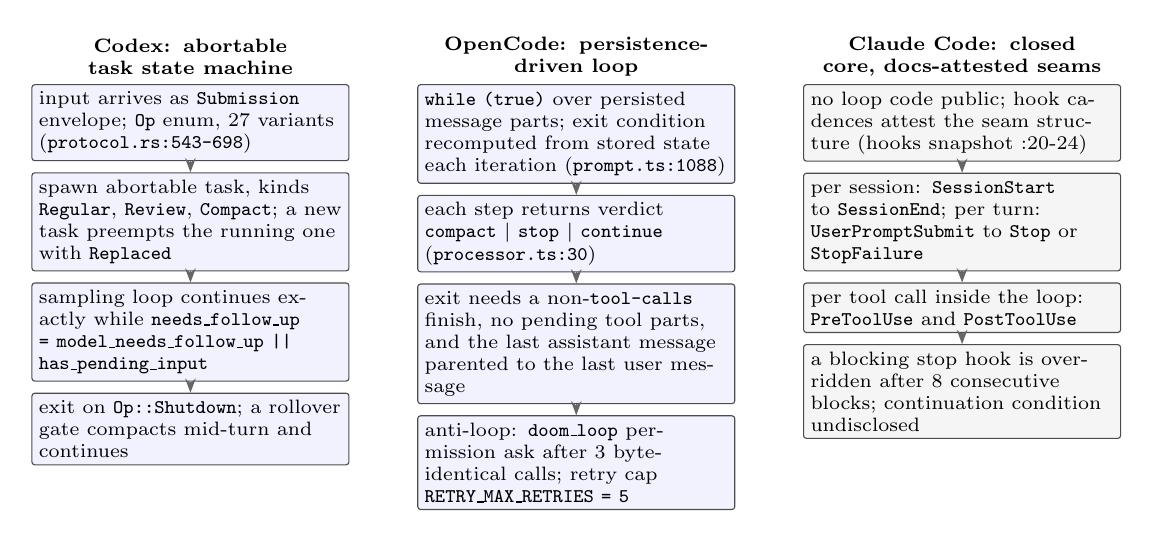
\begin{tikzpicture}[font=\scriptsize,
  head/.style={align=center, font=\scriptsize\bfseries, text width=3.9cm},
  sbox/.style={draw=black!70, rounded corners=1pt, align=left, anchor=north,
    text width=3.85cm, inner sep=2.5pt, fill=blue!5, text=black},
  csbox/.style={sbox, fill=gray!8},
  arr/.style={-{Stealth[length=1.8mm]}, draw=black!60, line width=0.5pt}]
% Codex column
\node[head] at (0,0.6) {\codex{}: abortable task state machine};
\node[sbox] (cx1) at (0,0.25) {input arrives as \texttt{Submission} envelope; \texttt{Op} enum, 27 variants (\texttt{protocol.rs:543-698})};
\node[sbox] (cx2) at ([yshift=-4pt]cx1.south) {spawn abortable task, kinds \texttt{Regular}, \texttt{Review}, \texttt{Compact}; a new task preempts the running one with \texttt{Replaced}};
\node[sbox] (cx3) at ([yshift=-4pt]cx2.south) {sampling loop continues exactly while \texttt{needs\_follow\_up = model\_needs\_follow\_up || has\_pending\_input}};
\node[sbox] (cx4) at ([yshift=-4pt]cx3.south) {exit on \texttt{Op::Shutdown}; a rollover gate compacts mid-turn and continues};
% OpenCode column
\node[head] at (4.9,0.6) {\occ{}: persistence-driven loop};
\node[sbox] (oc1) at (4.9,0.25) {\texttt{while (true)} over persisted message parts; exit condition recomputed from stored state each iteration (\texttt{prompt.ts:1088})};
\node[sbox] (oc2) at ([yshift=-4pt]oc1.south) {each step returns verdict \texttt{compact \textbar{} stop \textbar{} continue} (\texttt{processor.ts:30})};
\node[sbox] (oc3) at ([yshift=-4pt]oc2.south) {exit needs a non-\texttt{tool-calls} finish, no pending tool parts, and the last assistant message parented to the last user message};
\node[sbox] (oc4) at ([yshift=-4pt]oc3.south) {anti-loop: \texttt{doom\_loop} permission ask after 3 byte-identical calls; retry cap \texttt{RETRY\_MAX\_RETRIES = 5}};
% Claude Code column
\node[head] at (9.8,0.6) {\ccc{}: closed core, docs-attested seams};
\node[csbox] (cc1) at (9.8,0.25) {no loop code public; hook cadences attest the seam structure (hooks snapshot :20-24)};
\node[csbox] (cc2) at ([yshift=-4pt]cc1.south) {per session: \texttt{SessionStart} to \texttt{SessionEnd}; per turn: \texttt{UserPromptSubmit} to \texttt{Stop} or \texttt{StopFailure}};
\node[csbox] (cc3) at ([yshift=-4pt]cc2.south) {per tool call inside the loop: \texttt{PreToolUse} and \texttt{PostToolUse}};
\node[csbox] (cc4) at ([yshift=-4pt]cc3.south) {a blocking stop hook is overridden after 8 consecutive blocks; continuation condition undisclosed};
\draw[arr] (cx1.south) -- (cx2.north);
\draw[arr] (cx2.south) -- (cx3.north);
\draw[arr] (cx3.south) -- (cx4.north);
\draw[arr] (oc1.south) -- (oc2.north);
\draw[arr] (oc2.south) -- (oc3.north);
\draw[arr] (oc3.south) -- (oc4.north);
\draw[arr] (cc1.south) -- (cc2.north);
\draw[arr] (cc2.south) -- (cc3.north);
\draw[arr] (cc3.south) -- (cc4.north);
\end{tikzpicture}
\caption{The same abstract loop, three realizations. \codex{} and \occ{}
cells are code-anchored at the pinned commits; \ccc{} cells are
documentation-attested (shaded). Values match Table~\ref{tab:turnloop}.}
\label{fig:turnloops}
\end{figure}

\begin{table}[t]
\centering
\small
\caption{Turn-loop structures at the pinned commits. \ccc{} values are
docs-attested; its implementation values are undisclosed (closed core).}
\label{tab:turnloop}
\setlength{\tabcolsep}{4pt}%
\begin{tabular}{@{}L{\lblcol}L{\dimcol}L{\dimcol}L{\dimcol}@{}}
\toprule
Property & \codex{} & \occ{} & \ccc{} (docs)\\
\midrule
Realization & background Tokio task; \path{Submission} envelope; \path{Op} enum, 27 variants; loop exits on \path{Op::Shutdown} (\path{protocol.rs:543-698}) & \path{while (true)} over persisted message parts, \path{prompt.ts:1088} & closed; per-turn \path{UserPromptSubmit ... Stop/StopFailure} nesting per-tool-call \path{PreToolUse/PostToolUse} (hooks snapshot :20-24)\\
Continuation & \path{needs_follow_up = model_needs_follow_up || has_pending_input}, \path{session/turn.rs:405} & exit needs non-\path{tool-calls} finish, no pending tool parts, assistant parented to last user message (\path{prompt.ts:1106-1130}) & undisclosed\\
Step verdict & n/a (task-level: 3 \path{TaskKind} variants Regular, Review, Compact) & \path{compact|stop|continue}, \path{processor.ts:30} & undisclosed\\
Abort & 4 \path{TurnAbortReason} variants; spawn preempts with \path{Replaced} (\path{tasks/mod.rs:279-288}) & abort routes; denied permissions break the loop unless an experimental flag is set & undisclosed\\
Anti-loop & 8-variant \path{NotSubmittedReason} steering rejections (\path{turn_input.rs:182-208}) & \path{DOOM_LOOP_THRESHOLD = 3} byte-identical calls raise a permission ask (\path{processor.ts:29}) & stop hooks capped after 8 consecutive blocks (hooks snapshot :2397)\\
Retry and caps & n/a at loop level & \path{RETRY_MAX_RETRIES = 5}, initial delay 2000 ms, backoff factor 2 (\path{retry.ts:26-31}); per-agent \path{steps} cap is a soft guardrail & undisclosed; docs cap agent hooks at 50 turns (hooks snapshot)\\
\bottomrule
\end{tabular}
\end{table}

The design question a turn loop answers is: what keeps the loop going,
and what stops it from spinning. All three systems converge on the intent
of both answers and diverge in mechanism.

\codex{} answers with typed machinery and centralized control. Input
arrives as \path{Submission} envelopes whose \path{Op} enum has exactly 27
variants at the pinned commit; task spawning preempts any running task
with \path{TurnAbortReason::Replaced}; and the continuation condition is
one expression, \path{needs_follow_up = model_needs_follow_up ||
has_pending_input}, where the model-side bit is set by queued tool calls,
tool errors marked \path{RespondToModel}, and completed responses that did
not end the turn~\citep{codexRepo}. Steering an active turn is a typed
decision with an 8-variant rejection taxonomy: an accepted reply means
only that the core accepted the input for processing, not that it will
act on it. The reading of this design is a control plane culture: every
decision the loop can make is an explicit, enumerable
event~\citep{codexRepo}. Mid-turn, a rollover gate runs automatic
compaction before continuing, so compaction is a state transition inside
the turn rather than between turns (Section~\ref{sec:compaction}).

\occ{} takes the opposite position: the loop's truth lives in storage.
Rather than tracking step state in memory, it recomputes its exit
condition each iteration from persisted message parts; exiting requires
all of a non-\path{tool-calls} finish reason, no pending tool parts, and
the last assistant message parented to the last user message, and the
exit-condition comment explains the redundancy as defense against
providers that return \path{stop} while tool calls are still
queued~\citep{opencodeRepo}. Each step returns one of three
verdicts, \path{compact}, \path{stop}, or \path{continue}, so the loop
and the context manager share one vocabulary. The anti-loop defense is
behavioral rather than structural: three byte-identical calls of one tool
raise a \path{doom_loop} permission ask whose default action is itself
\path{ask}~\citep{opencodeRepo}. The reading is a storage-first culture:
make the loop honest about what it persisted, and let the user arbitrate
the edge cases.

\ccc{} exposes no loop code, and the only numeric constant its
documentation discloses is the seam behavior: hook cadences run once per
session, once per turn, and on every tool call inside the agentic loop,
and a blocking stop hook is overridden after 8 consecutive
blocks~\citep{claudeCodeHooksDocs}. The cadences attest that a loop with
that nesting structure exists; the continuation condition, any step cap,
and the retry policy are not documented
(Section~\ref{sec:limitations}).

\subsection{Tool surfaces and patch application}
\label{sec:tools}

The tool shapes overlap (one shell path, at least one edit path, search,
delegation), but the registration policy and the edit protocol differ
(Table~\ref{tab:tools}).

\begin{table}[t]
\centering
\small
\caption{Tool surfaces. \codex{} and \occ{} cells are code-anchored; \ccc{}
cells are docs-attested or attested by the pinned plugin surface (closed
core). Undisclosed cells have no pinned source.}
\label{tab:tools}
\setlength{\tabcolsep}{4pt}%
\begin{tabular}{@{}L{1.7cm}L{3.75cm}L{3.75cm}L{3.75cm}@{}}
\toprule
Shape & \codex{} & \occ{} & \ccc{} (docs/surface)\\
\midrule
Shell & \path{shell_command} (legacy) or \path{exec_command} + \path{write_stdin} (unified pty), chosen by shell tool type & \path{bash} & \path{Bash}, plus \path{PowerShell} (hooks snapshot :1513)\\
File edit & \path{apply_patch}, freeform string parsed by a 19-line Lark grammar & \path{edit} (9-stage replacer cascade, similarity 0.65) and \path{write}; \path{apply_patch} port & \path{Edit}, \path{Write}, \path{MultiEdit}, \path{NotebookEdit} (surface attestations)\\
Patch-vs-edit choice & gated on \path{model_info.apply_patch_tool_type} & \path{apply_patch} replaces \path{edit}/\path{write} for \path{gpt-*} except \path{gpt-4}/\path{oss} (\path{registry.ts:296-300}) & undisclosed\\
Read/search & no dedicated tools; shell carries read and search; \path{view_image} for images & \path{read}, \path{glob}, \path{grep} & \path{Read}, \path{Glob}, \path{Grep} (hooks snapshot :1513)\\
Delegation & 6 v2 agent tools (\path{spawn_agent} ... \path{list_agents}) or 5 v1 tools, feature-gated & \path{task} & \path{Agent} (docs), \path{Task} (surface); \path{SubagentStart/Stop} hook events\\
Planning & \path{update_plan} behind config & \path{plan_exit} behind experimental flags & \path{ExitPlanMode} (hooks snapshot :1513)\\
Discovery & \path{tool_search} registered only when a deferred searchable tool exists & none builtin & \path{ToolSearch} enabled by default; doubles as the MCP wait point (MCP snapshot :279,:310)\\
Context tooling & \path{new_context} and \path{get_context_remaining} behind a feature gate & session-managed compaction, no model-visible tool & no model-visible tool attested; \path{PreCompact/PostCompact} hook seams\\
Shell defaults & 10 s timeout, 1 MiB output cap, 10{,}000 event deltas per call; unified exec: 10 s yield default clamped at 30 s, 300 s background, 64 processes & truncation via \path{tool/truncate.ts}; numeric caps outside E2 scope & Bash sandbox scope is Bash-only (surface); numeric defaults undisclosed\\
\bottomrule
\end{tabular}
\end{table}

The design question SWE-agent's results raise is not just which tools
exist, but what the edit protocol looks like, since free-form shell
editing is the failure-prone baseline~\citep{yang2024sweagent}.

The inventory matters less than the policy behind it. \codex{} computes
its surface per turn: 32 conditional registrations, each gated on feature
flags, model capabilities, or the presence of other tools, so the set of
tools the model sees is itself derived
state~\citep{codexRepo}. \occ{} ships a fixed, ordered array of 17 tool
IDs: the surface is a constant~\citep{opencodeRepo}. \ccc{}'s registry is
only attestable through documentation (12 built-ins named in the hooks
snapshot plus MCP tools) and the pinned surface (8 more names, including
TodoWrite and Task), with the full closed-core inventory
open~\citep{claudeCodeHooksDocs,claudeCodeSurface}. Even discovery, where
it exists, is implemented differently: \codex{} registers
\path{tool_search} only when a deferred searchable tool exists, while
\ccc{} documents \path{ToolSearch} as enabled by default and as the point
where the harness waits for MCP
connections~\citep{codexRepo,claudeCodeMcpDocs}.

The most concrete cross-vendor artifact in the study is the patch format.
\codex{}'s \path{apply_patch} is a grammar-constrained freeform tool,
parsed by a 19-line Lark grammar; \occ{} ports that grammar essentially
verbatim (the port's comment reads ``Core types matching the Rust
implementation'', \path{patch/index.ts:12}) and swaps it in for
\path{edit} and \path{write} whenever the model ID contains
\path{gpt-}, except \path{gpt-4} and
\path{oss}~\citep{codexRepo,opencodeRepo}. Wire-format convergence is
happening even while control flow diverges. Part II turns out to hinge on
this same gate: the patch-versus-edit choice is exactly what changes when
the model stops being the vendor's own
(Sections~\ref{sec:compatcodex},~\ref{sec:compatopencode}).

Both open systems engineer around the edit-fragility that SWE-agent
measured, in different places. \occ{} runs its \path{edit} tool through a
9-stage fuzzy replacer cascade (Levenshtein similarity 0.65) to recover
from exactly the class of failure after which success probabilities drop
sharply~\citep{yang2024sweagent,opencodeRepo}; \codex{} instead
constrains the edit surface itself to a grammar and delegates file
inspection to its shell tool, shipping no dedicated read, glob, or grep
tools within the extracted registry~\citep{codexRepo}. Third-party
teardowns assert a larger \ccc{} inventory (49 tools in one binary
analysis) and a tool-tier design, but these remain unverified blog-tier
observations~\citep{tenguDecoded,minusXTeardown}.

\subsection{Context compaction}
\label{sec:compaction}

Both open systems trigger compaction at literal constants, and the
constants are of different kinds (Table~\ref{tab:compaction}).

\begin{table}[t]
\centering
\small
\caption{Compaction parameters at the pinned commits. \ccc{} exposes the
compaction lifecycle at hook seams but discloses no numeric thresholds in
the pinned snapshot set.}
\label{tab:compaction}
\setlength{\tabcolsep}{4pt}%
\begin{tabular}{@{}L{\lblcol}L{\dimcol}L{\dimcol}L{\dimcol}@{}}
\toprule
Parameter & \codex{} & \occ{} & \ccc{} (docs)\\
\midrule
Trigger style & fractional & reserved buffer & undisclosed\\
Threshold & 9/10 of the resolved context window, capped by config (\path{openai_models.rs:488-499}) & count reaches input limit minus a reservation defaulting to min(20{,}000, \path{maxOutputTokens}) tokens (\path{overflow.ts:8-34}) & undisclosed\\
Headroom & 95\% effective window default (\path{openai_models.rs:376-378}) & \texttt{COMPACTION\_BUFFER} = 20{,}000 tokens & undisclosed\\
Summary budget & user messages capped at 20{,}000 tokens locally (\path{compact.rs:57}) & pruning targets tool outputs, not user messages & undisclosed; root CLAUDE.md re-injected after \path{/compact}, nested files are not (memory snapshot :450-454)\\
Retention & remote path retains 64{,}000 tokens, agent messages capped at 10{,}000, 2 retries (\path{compact_remote_v2.rs:65-69}) & preserve clamp(25\% of usable, 2{,}000 to 15{,}000) tokens of recent messages (\path{compaction.ts:115-118}) & undisclosed\\
Pruning & summary replaces context; rollback op drops last N turns & keep last 40{,}000 tokens of tool output (\path{PRUNE_PROTECT}); minimum 20{,}000 before pruning; truncated outputs keep 2{,}000 chars; skill outputs never pruned & \path{PostCompact} input carries \path{compact_summary} (hooks docs)\\
Mid-turn & rollover runs auto-compaction then continues (ContextLimit, MidTurn) & verdict \path{compact} appends a compaction part and continues (\path{processor.ts:679}) & blocking \path{PreCompact} during context-limit recovery surfaces the error (hooks docs)\\
Token accounting & model-reported counts & chars/4 estimate for unknown counts (\path{token.ts:3-5}) & undisclosed\\
\bottomrule
\end{tabular}
\end{table}

Context is finite and every coding conversation grows, so a harness must
decide when the budget is exhausted and what to keep. The two trigger
philosophies visible in the pinned trees are the obvious two: fire at a
fraction of the window, or reserve a fixed headroom and fire when it is
eaten.

\codex{} uses the fraction. Compaction fires at nine tenths of the
resolved context window, on top of an effective window already held at
95\% of nominal, so the trigger is a proportion rather than a number and
tracks model capability automatically~\citep{codexRepo}. The summarizer
itself is budgeted: 20{,}000 tokens of user messages locally, and on the
remote path 64{,}000 tokens of retention with 10{,}000-token agent
message caps and 2 retries. Because the rollover gate can fire mid-turn,
compaction is a state transition inside the turn rather than a pause
between turns.

\occ{} uses the reservation: overflow fires when the running token count
reaches the input limit minus a reserved buffer defaulting to
min(20{,}000, \path{maxOutputTokens})
tokens~\citep{opencodeRepo}. More instructive than the trigger is what
the budgets protect. They are pruning-shaped rather than summary-shaped,
and aimed at tool output, where a coding agent's context actually bloats:
keep the last 40{,}000 tokens of tool output, only prune when at least
20{,}000 tokens exist, truncate outputs to 2{,}000 characters, never prune
skill outputs, and retain recent messages clamped to 25\% of the usable
window within 2{,}000 to 15{,}000 tokens. Unknown counts are estimated
as characters divided by four.

\ccc{} documents the lifecycle but not the numbers. Hooks carry
\path{PreCompact}/\path{PostCompact} events with \path{manual}/\path{auto}
trigger values, and a hook blocking compaction during context-limit
recovery surfaces the underlying error; the memory documentation states
that project-root CLAUDE.md survives \path{/compact} by being re-read and
re-injected, while nested CLAUDE.md files do
not~\citep{claudeCodeHooksDocs,claudeCodeMemoryDocs}. No numeric trigger,
summarization budget, or retention policy appears anywhere in the pinned
snapshot set (Section~\ref{sec:limitations}). With open models, these
constants only matter once the accounting inputs are correct: Part II
shows each system mis-accounting in a different way when the model on the
other end is unknown to the harness
(Section~\ref{sec:matrix}).

\subsection{Permissions and sandboxing}
\label{sec:safety}

The three systems occupy three distinct points on the same axis
(Table~\ref{tab:safety}).

\begin{table}[t]
\centering
\small
\caption{Safety policies. \ccc{} cells cite the pinned documentation
snapshots and the pinned settings surface; enforcement internals are closed.
Undisclosed cells have no pinned source.}
\label{tab:safety}
\setlength{\tabcolsep}{4pt}%
\begin{tabular}{@{}L{\lblcol}L{\dimcol}L{\dimcol}L{\dimcol}@{}}
\toprule
Dimension & \codex{} & \occ{} & \ccc{} (docs)\\
\midrule
Policy engine & Starlark rule engine over \path{.codexpolicy} files & in-process permission ruleset & permission rules plus OS sandbox as two documented layers (sandboxing snapshot :521-525)\\
Decision model & \path{Decision = Allow|Prompt|Forbidden} (\path{decision.rs:9-16}) & \path{allow|ask|deny} per ruleset entry & six modes default, acceptEdits, plan, auto, dontAsk, bypassPermissions (permissions snapshot :56-63); rule order deny, ask, allow (:42)\\
Aggregation & strictest-wins via \path{max()} over matched rules (\path{policy.rs:402-403}) & merge precedence not extracted & hook decisions \path{deny > defer > ask > allow} (hooks docs)\\
Shipped content & no \path{.rules} file; only a 78-line example marked not recommended for actual use & default ruleset ships: \path{"*": allow}, doom loop ask, \path{question/plan_enter/plan_exit} deny, \path{*.env} ask (\path{agent.ts:119-136}) & rule syntax documented; no shipped default policy text in snapshots\\
OS sandbox & Seatbelt (macOS, 122-line compiled policy), bubblewrap argv plus seccomp/landlock network filtering (Linux) & none found in the pinned tree & built-in Seatbelt (macOS); bubblewrap plus socat (Linux, WSL2); native Windows not supported (sandboxing snapshot)\\
Sandbox scope & 4 \path{SandboxPolicy} variants; \path{WritableRoot} protects \path{.git}, \path{.agents}, \path{.codex} (\path{protocol/src/permissions.rs:24-33}) & n/a & Bash commands and their child processes only; Read/Edit/Write use the permission system directly (sandboxing snapshot :523,:658)\\
Network control & seccomp denies ptrace/\path{io_uring}; restricted mode denies sockets except \path{AF_UNIX} & n/a & no domains pre-allowed; first connection prompts; allow for the session (sandboxing docs)\\
Evasion resistance & 90-line banned list of amendable shell/runtime prefixes (\path{exec_policy.rs:58-147}) & bash arity normalization, longest-prefix-wins over about 130 entries, before rule matching & fixed wrapper stripping; argument-scoped allow patterns documented as fragile (permissions snapshot)\\
Kill switches & enterprise \path{requirements.toml}; trust gating of project config & environment flags & \texttt{disable\-Bypass\-Permissions\-Mode} and \texttt{disable\-Auto\-Mode} (permissions snapshot :69)\\
\bottomrule
\end{tabular}
\end{table}

Every coding agent eventually hands the model a way to run code on a
machine, so every harness must answer one question: what stops a bad
command? The three systems are three canonical answers: prevent, recover,
and layer.

\codex{} prevents. Shell access is wrapped in an OS sandbox per platform
(a 122-line Seatbelt policy compiled into the binary on macOS, and a
bubblewrap argument builder plus seccomp filter denying ptrace and
\path{io_uring} on Linux) under a Starlark rule engine that evaluates
each command with a three-valued decision and strictest-wins
aggregation~\citep{codexRepo}. Two choices are worth noting as a learning
point. First, no policy file ships with the repository (the only example
is labeled as not recommended for actual use), so the default is
approval-driven rather than policy-driven: the machinery is deep but
idle until a user supplies rules. Second, writable roots still deny writes
to harness metadata (\path{.git}, \path{.agents}, \path{.codex}), and command
injection is addressed with a static 90-line list of amendable shell and
runtime prefixes~\citep{codexRepo,codexSandboxingDocs}.

\occ{} recovers. All safety is in-process: the pinned tree contains no OS
sandbox machinery within the searched scope, and the default ruleset is
\path{"*": allow}, with friction narrowed to dot-env reads (ask), the
doom-loop tripwire (ask), external directories (ask), and denials for the
interaction and plan tools. Its answer to command smuggling is
normalization: shell commands are reduced to canonical arity by a
longest-prefix-wins dictionary of about 130 entry types before rules
match~\citep{opencodeRepo,opencodeDocs}. The permissive default is not
carelessness; it is paired with a recovery budget that the other two
systems lack, per-step file snapshots with revert
(Section~\ref{sec:state}). A user can undo anything the agent did, so the
harness risks more by default.

\ccc{} layers. Permission rules are evaluated before any tool runs, in a
fixed order of deny, then ask, then allow, and the OS sandbox ``applies
only to Bash commands and their child processes'', while Read, Edit, and
Write ``use the permission system
directly''~\citep{claudeCodePermissionsDocs,claudeCodeSandboxingDocs,%
claudeCodeHooksDocs}. The scope choice is deliberate and instructive:
capability (file tools that run unsandboxed) is traded against a narrow,
strongly enforced shell boundary, since the shell is the surface where
arbitrary execution actually lives. Enforcement is platform-native
(Seatbelt on macOS, bubblewrap plus socat on Linux and WSL2), no network
domain is pre-allowed, protected paths such as the client's settings, git
hooks, and shell startup files are denied writes even inside writable
roots with no per-path exemption, and enterprise kill switches disable
the bypass and auto modes. The pinned surface adds the reference
confinement for untrusted work: a devcontainer whose firewall defaults to
dropping egress outside an allowlist~\citep{claudeCodeSurface}. The
implementation of these layers is closed (Section~\ref{sec:limitations}).

\subsection{Extensibility}
\label{sec:extensibility}

The vocabulary has converged: all three expose hooks, plugins, skills,
agents or subagents, and MCP integration. The real design difference is
the trust model: extension code is another person's program, and each
system draws a different line around how much privilege it
deserves~\citep{codexRepo,opencodeRepo,claudeCodePluginsDocs}.

\codex{} treats hook code as untrusted input. Handlers are content-hashed
and run only when marked managed or trusted, so a pull request that edits
a workflow is detectable at the trust boundary. Hooks are external
processes (11 events, regex matchers); \path{PreToolUse} can block,
inject context, or rewrite tool input, with exit code 2 as the block
signal. Plugins are \path{<plugin>@<marketplace>} packages discovered
under \path{.codex-plugin}, \path{.claude-plugin}, and
\path{.cursor-plugin} layouts, and the \ccc{} compatibility is explicit:
plugin environments export \path{CLAUDE_PLUGIN_ROOT} and
\path{CLAUDE_PLUGIN_DATA} ``for OOTB compat with existing plugins''.
Skills are markdown documents budgeted at 2\% of the context window,
capped at 10{,}000 tokens.

\occ{} takes the maximal-trust position: plugins are in-process
TypeScript functions sharing the harness's own API surface, dispatched
sequentially in registration order; ten of the eleven internal plugins
are provider authentication bundles built on the same mechanism. It also
uses the plugin API for itself, defining seven built-in agents, including
dedicated compaction, title, and summary agents, with \path{explore}
read-only by ruleset except an explicit \path{bash: "allow"}
(\path{agent.ts:205}). The tradeoff is visible in the trust surface:
plugins receive the full SDK client in-process, and the SDK declares a
\path{permission.ask} hook for which no trigger call site exists at this
commit. Skills are discovered from the native, the vendor-neutral
\path{.agents}, and the \ccc{} \path{.claude} layouts, and each doubles
as a slash command~\citep{opencodeRepo,opencodeDocs}.

\ccc{} documents the broadest lifecycle: 31 hook events with five handler
types (command, HTTP, MCP tool, prompt, agent), hooks running in
parallel, and agent hooks capped at 50 turns; plugins carry up to ten
component kinds, including monitors and bundled executables, distributed
through two public marketplaces, one curated and one community-reviewed;
subagents are quota-controlled by documentation, with a default depth of
three layers, a 20-concurrent cap, and forks that inherit the full
conversation but cannot spawn further
forks~\citep{claudeCodeHooksDocs,claudeCodePluginsDocs,%
claudeCodeSubagentsDocs}. The learning point is how much power the
documented contract already carries: the pinned surface contains an
unbounded autonomous-loop plugin implemented entirely as a shell script
that repeatedly blocks the Stop event (the ralph-wiggum plugin), with no
core changes at all~\citep{claudeCodeSurface}. A good contract can replace
a plugin API.

\subsection{Configuration and providers}
\label{sec:config}

Configuration precedence answers a security question wearing a
convenience costume: when the repository, the user, and the enterprise
disagree about a setting, who wins? Each system turns the answer into an
explicit ordered merge and, more tellingly, a judgment about what
repository content may ever override.

\codex{} ranks ten provenance layers numerically (packaged defaults at
the bottom at -10, MDM-delivered managed config at the top at 50) with
recursive table merging in which overlays replace non-table values
wholesale and arrays never union~\citep{codexRepo}. Two couplings to
safety are the lesson. Project-local configuration is disabled until the
project is trusted, and a twelve-key denylist hard-blocks repository
content from setting provider endpoints, model providers, notification,
profile, realtime, and telemetry keys, with the source comment that
repo-local config should not choose where credentials are
sent~\citep{codexRepo}. The provider layer is deliberately narrow:
exactly five built-in provider IDs, reserved against override except
Bedrock, and a wire protocol pinned to the Responses API, with the legacy
chat protocol rejected as a hard error.

\occ{} takes the opposite bet, capability first. Its nine-layer chain
ends in admin-managed config directories and a macOS MDM plist whose code
comment states it overrides everything, with one asymmetry that shows
where the designers' attention went: inside \path{.opencode} directories,
the entry farther from the working directory wins, the opposite of
plain-file precedence~\citep{opencodeRepo}. The provider layer is the
widest of the three: 24 bundled provider packages, runtime installation
of arbitrary provider SDKs named in config, and a hosted catalog fetched
from models.opencode.ai and cached for five minutes. The cost of that
openness is a permissive configuration parser: unknown keys are silently
discarded, environment substitution falls back to empty without error,
and an inline environment variable replaces the credentials file without
schema validation.

\ccc{}'s loader is closed, but the documented contract makes its most
instructive distinction explicit: guidance versus enforcement. CLAUDE.md
files shape behavior but ``are not a hard enforcement layer'', while
settings rules are enforced by the client regardless of model behavior,
and managed-policy memory files are non-excludable and load
first~\citep{claudeCodeMemoryDocs}. The split explains the system's trust
shape: advisory context for the model, hard rules around it. MCP servers
follow a five-level scope precedence (local, project, user, plugin,
connector) taken wholesale without field merging, and project-scoped
\path{.mcp.json} servers require approval and are gated on workspace
trust~\citep{claudeCodeMcpDocs}.

Part II is this dimension under stress: the provider-plumbing culture
each system built here is precisely what decides how far open-weight
models get (Sections~\ref{sec:compatcodex}
to~\ref{sec:compatccc}).

\subsection{State, rollout, and interfaces}
\label{sec:state}

Session state answers the durability question: how much of a session
survives, and how exactly can it be resumed? The two open answers embody
opposite bets on where the source of truth should live.

\codex{} bets on inspectability. Each thread persists as append-only,
human-readable JSONL under a dated directory, with a head metadata record
and per-record flushes; six SQLite databases mirror thread metadata but
are treated as repairable caches, falling back to filesystem read-repair;
cold rollouts are zstd-compressed after seven days~\citep{codexRepo}. The
payoff is the resume path: reconstruction reverse-scans to a compaction
base and replays forward, honoring rollbacks, so resume is exact across
compaction boundaries rather than approximate. Offline memories are
generated from the same rollouts, making the conversation log the
machine's single source of truth about itself.

\occ{} bets on recoverable mistakes. Sessions live in SQLite tables
written exclusively by event projectors over a durable event log with
contiguous per-aggregate sequence numbers, and file history is separated
from conversation history: snapshots are git tree objects in a shadow
repository (never commits), captured before streaming starts and at every
step boundary, and reverted by checking out saved hashes in batches of
100 files, with a 2 MiB untracked-file cap~\citep{opencodeRepo}. This is
the other half of the safety argument from
Section~\ref{sec:safety}: permissive defaults are affordable because any
step can be undone file-by-file. Sharing syncs a session to a public URL;
projects that are not git repositories get no snapshot tracking.

\ccc{} session storage is not inspectable. Documentation attests
per-subagent transcripts retained across restarts within a session and
deleted after a 30-day default cleanup, and notes that the transcript
handoff to hooks ``may lag'' the in-memory conversation, which is itself
a statement about where the truth
lives~\citep{claudeCodeSubagentsDocs,claudeCodeHooksDocs}.

Interfaces answer a smaller question with large consequences: how many
sources of truth exist for the agent's surface? \codex{} keeps exactly
one: TUI, headless exec, and the app and exec servers are all clients of
one JSON-RPC protocol, approvals are server-to-client requests,
backpressure has a dedicated error code (-32001), and headless exec
refuses to run outside a git repository unless explicitly
overridden~\citep{codexRepo}. \occ{} runs the reverse of a monolith: the
TUI is a client of a local HTTP server exposing the full surface (prompt,
summarize, fork, abort, share, revert), plus an Agent Client Protocol
implementation, plus 38 built-in LSP servers whose severity-one
diagnostics are fed back into edit tool outputs. The LSP feedback is a
closed loop from checker to model, the closest thing in the study to
SWE-agent's lint gating shipped as
infrastructure~\citep{opencodeRepo,yang2024sweagent}. \ccc{} documents
CLI, IDE extensions, desktop, and four MCP transports; the reference
confinement for untrusted work is a firewalled
devcontainer~\citep{claudeCodePermissionsDocs,claudeCodeMcpDocs,%
claudeCodeSurface}.

\part{Open-source model support}

\section{The compatibility question}
\label{sec:compatintro}

Whether a given harness supports open-source models is a concrete,
answerable question: does the provider plumbing know about local servers,
what wire protocol does it speak, and what degrades when the model on the
other end is not the vendor's own? The question has three surfaces to
hold constant while the agent varies: Ollama, LM Studio, and the generic
OpenAI-compatible server class embodied by the llama.cpp reference
server~\citep{ollamaCompatDocs,lmstudioApiDocs,llamaCppServerDocs}. We
also ask the mirror question: what must a compatible server provide for
an agent to survive against it?

Part II is a static source trace under the same discipline as Part I:
nothing was executed, no model API was called, and provider behavior is
stated only as code paths and documentation contracts. Where a system's
behavior is closed or unattested, the cell says so
(Section~\ref{sec:limitations}).

\subsection{What the servers themselves provide}
\label{sec:servers}

The compatibility bar is set by what a compatible server can actually
do (Table~\ref{tab:servers}, Figure~\ref{fig:protocolbar}).

\begin{table}[t]
\centering
\small
\caption{Server-side contract, from each reference server's own
documentation snapshots. Responses: whether an OpenAI Responses API
route exists and how it is described.}
\label{tab:servers}
\setlength{\tabcolsep}{4pt}%
\begin{tabular}{@{}L{1.7cm}L{3.9cm}L{3.9cm}L{3.5cm}@{}}
\toprule
Server & Baseline OpenAI surface & Tool calling & Responses API\\
\midrule
Ollama (2024 post) & \path{/v1/chat/completions} at \path{localhost:11434}; auth placeholder ``required, but unused'' (\texttt{ollama\-Compat\-Docs}) & listed as a possible future improvement at post time & not mentioned\\
LM Studio & chat completions and more at \path{localhost:1234/v1} (\path{lmstudio\-Api\-Docs}) & on \path{/v1/chat/completions}; parallel calls and \path{tool_choice} undocumented; streaming deltas indexed & route exists; docs cover streaming, \path{reasoning.effort}, \path{previous_response_id}, remote MCP tools; no function tools documented on that page\\
llama.cpp reference server & models, completions, chat completions, embeddings, plus health, props, metrics, slots; self-described: ``no strong claims of compatibility'' & template-gated via \path{--jinja}; \path{parallel_tool_calls} ``only supported on some models'' & exists but is a converter stub into chat completions; no streaming or tools documented for the route\\
\bottomrule
\end{tabular}
\end{table}

\begin{figure}[t]
\centering
\begin{tikzpicture}[font=\scriptsize, scale=0.92, transform shape,
  proto/.style={draw=black!70, line width=0.7pt, rounded corners=1pt,
    fill=black!5, align=center, minimum width=3.85cm, minimum height=0.95cm,
    inner sep=2.5pt, text=black},
  reqlab/.style={draw=black!40, line width=0.5pt, rounded corners=1pt,
    align=center, minimum width=3.85cm, minimum height=0.85cm,
    inner sep=2.5pt, text=black},
  chip/.style={rounded corners=1pt, align=center, minimum width=3.85cm,
    minimum height=0.85cm, inner sep=2.5pt, text=black},
  rowhead/.style={draw=black!50, line width=0.5pt, rounded corners=1pt,
    fill=black!5, align=center, minimum width=2.3cm, inner sep=2.5pt,
    text=black},
  arr/.style={-{Stealth[length=1.8mm]}, draw=black!60, line width=0.5pt}]
% protocol columns
\node[proto] (p1) at (0,0) {\textbf{Chat completions}\\ plus tool calls};
\node[proto] (p2) at (4.25,0) {\textbf{Responses API}\\ (OpenAI)};
\node[proto] (p3) at (8.5,0) {\textbf{Anthropic}\\ \path{/v1/messages}};
% agent requirements
\node[reqlab, fill=genericcol!14] (oc) at (0,1.75) {\occ{} accepts any\\ chat-completions shape};
\node[reqlab, fill=nativecol!14] (cx) at (4.25,1.75) {\codex{} pins Responses;\\ \path{chat} is a hard error};
\node[reqlab, fill=unattcol!14] (ccreq) at (8.5,1.75) {\ccc{}: Anthropic protocol\\ only, as attested};
\draw[arr] (oc.south) -- (p1.north);
\draw[arr] (cx.south) -- (p2.north);
% Ollama row
\node[rowhead] at (-3.0,-1.4) {Ollama\\ 2024 snapshot};
\node[chip, fill=partcol!16] at (0,-1.4) {partial: chat yes, tools\\ listed as future};
\node[chip, fill=black!7] at (4.25,-1.4) {absent: not in snapshot};
\node[chip, fill=black!7] at (8.5,-1.4) {absent: not in snapshot};
% LM Studio row
\node[rowhead] at (-3.0,-2.5) {LM Studio\\ docs mirror};
\node[chip, fill=genericcol!14] at (0,-2.5) {supported: tools on chat\\ completions; no parallel flag};
\node[chip, fill=partcol!16] at (4.25,-2.5) {partial: streaming, effort,\\ prior state, remote MCP only};
\node[chip, fill=black!7] at (8.5,-2.5) {named only: shape\\ undocumented};
% llama.cpp row
\node[rowhead] at (-3.0,-3.6) {llama.cpp\\ reference server};
\node[chip, fill=genericcol!14] at (0,-3.6) {supported: tools via\\ jinja templates, JSON schema};
\node[chip, fill=partcol!16] at (4.25,-3.6) {partial: documented as a\\ converter to chat completions};
\node[chip, fill=genericcol!14] at (8.5,-3.6) {supported:\\ \path{/v1/messages} documented};
\end{tikzpicture}
\caption{Wire protocols as a compatibility bar. Top row: the protocol each
agent commits to. Bottom grid: what each reference server documents for
that protocol. Every status is written into its chip; shading only
repeats the status.}
\label{fig:protocolbar}
\end{figure}

Two readings matter for the agents. First, the practical minimum for a
coding agent is chat completions with tool calling; streaming is a
comfort feature, and structured output support is uneven. Second, the
Responses API surface is young and incomplete everywhere it exists: an
agent that pins itself to Responses (Section~\ref{sec:compatcodex}) is
betting on servers catching up. A separate fact becomes relevant in
Section~\ref{sec:compatccc}: the llama.cpp reference server also exposes
an Anthropic-shaped \path{/v1/messages} route, and LM Studio documents an
Anthropic-compatible surface~\citep{llamaCppServerDocs,lmstudioApiDocs}.

\subsection{Codex: a first-class Responses path, with caveats}
\label{sec:compatcodex}

\codex{}'s answer is structural: Ollama and LM Studio are not generic
endpoints bolted on, they are provider entries. Both are registered with
the responses wire type, and all model traffic is
\path{POST <base_url>/responses}, \path{http://localhost:11434/v1/responses}
and \path{http://localhost:1234/v1/responses}
(\path{codex-rs/model-provider-info/src/lib.rs:514-521},
\path{codex-rs/codex-api/src/endpoint/responses.rs:100-102}). The
legacy chat wire is not a fallback: setting \path{wire_api = "chat"} is a
hard deserialization error~\citep{codexRepo}.

Three design details shape the experience. \emph{Version gating}: before
use, \codex{} probes Ollama with \path{GET /api/version} and refuses
servers that report a version older than 0.13.4, except dev builds that
report \path{0.0.0} and servers whose version endpoint is missing or
unparsable; the gate is consistent with Responses support landing in
later Ollama releases, although the code does not state the
reason~\citep{codexRepo,ollamaCompatDocs}. \emph{Logistics}: the LM
Studio client probes \path{GET <base>/models}, downloads via
\path{lms get --yes}, and warms up with a one-token responses request;
the Ollama client pulls models over the native \path{/api/pull} NDJSON
stream, reading success from the event stream rather than the HTTP
status~\citep{codexRepo}. \emph{Defaults}: the default models are
\path{gpt-oss:20b} (Ollama) and \path{openai/gpt-oss-20b} (LM Studio),
slugs from the gpt-oss open-weight family~\citep{codexRepo}.

The caveats are equally structural. Those default slugs are absent from
the bundled catalog, so, provided the catalog refresh does not decode a
richer listing from the server, they resolve to a fallback model
description with no patch tool type, and the \path{apply_patch} tool is
registered only when that type is set: open models on \codex{} lose the
patch tool, while the rest of the registry is gated by feature and
environment rather than provider~\citep{codexRepo}. Requests to local
servers still carry the full field set, tools JSON,
\path{tool_choice: "auto"}, \path{parallel_tool_calls}, schema-shaped
output, \path{reasoning.summary} defaulting to auto, and
\texttt{include: ["reasoning.encrypted\_content"]}; the server-side
acceptance of each field is not checkable from either side of this
trace~\citep{codexRepo,lmstudioApiDocs,llamaCppServerDocs}. Unknown
models inherit, under the same fallback proviso, a context accounting
of 272{,}000 tokens unless the user sets
\path{model\_context\_window}, and overrides exist via
\path{CODEX\_OSS\_BASE\_URL} and \path{CODEX\_OSS\_PORT}; no OSS provider
entry carries authentication~\citep{codexRepo}.

\subsection{OpenCode: generic compatibility, permissive defaults}
\label{sec:compatopencode}

\occ{} has the widest answer and the sharpest degradations. Any provider
it does not know rides the generic OpenAI-compatible SDK: the factory is
one of 24 bundled provider packages and is also the final fallback for
catalog models and config-defined
models~\citep{opencodeRepo}. The user-facing shape is a config
block, \path{provider.<id>} with \path{options.baseURL} and
\path{options.apiKey} plus per-model limits; an in-repo test example
runs exactly the Ollama setup, \path{baseURL "http://localhost:11434/v1"}
with limits context 8192, output 2048. Custom SDKs install at runtime
from \path{npm}, or from a local path via \path{file://}, and the hosted
catalog at models.opencode.ai (five-minute cache, overridable and
disablable by flags) lists, in the pinned test fixture, an
\path{lmstudio} provider at \path{http://127.0.0.1:1234/v1} and an
\path{ollama-cloud} provider, though no bare local Ollama
entry~\citep{opencodeRepo}.

The degradations follow from the defaults. An unconfigured limit is
zero: output limit zero silently becomes the 32{,}000-token request cap
(\path{OUTPUT\_TOKEN\_MAX}), and context limit zero disables
auto-compaction entirely, so a local session can drive straight into the
wall without the harness budgeting anything~\citep{opencodeRepo}. Token
counts for unknown models are estimated as characters over four; the
compaction reserve on the v1 overflow path, when it runs, is
min(20{,}000 tokens, \path{maxOutputTokens}); a second compaction path
exists in the pinned tree and which one serves the default run is
unresolved~\citep{opencodeRepo}. Tools are sent unconditionally with the
capability flag defaulting to true, so a server without tool support is
not discovered until the request fails, or, worse, the model simply
never calls a tool and file editing quietly
disappears~\citep{opencodeRepo}. An unknown model string is a hard error
with fuzzy suggestions rather than a silent fallback, which is honest but
unforgiving~\citep{opencodeRepo}. Two filters shape what open models
see: \path{websearch} is dropped for every provider except the native
ones, and the model-ID-keyed choice is the edit path, the
\path{apply\_patch} port is gated to model IDs containing \path{gpt-},
excluding \path{gpt-4} and \path{oss}, so open models get the
\path{edit} and \path{write} tools instead~\citep{opencodeRepo}.

\subsection{Claude Code: no documented surface, and a gray zone}
\label{sec:compatccc}

The documentation snapshots are unambiguous about what is supported:
Anthropic-model clouds. The model page covers aliases, version pins, and
provider-specific resolution across Anthropic's own infrastructure,
Bedrock, Google's Agent Platform, and partner clouds, and the Bedrock
page wires Claude Code to AWS with \path{CLAUDE\_CODE\_USE\_BEDROCK=1};
every documented model example there is an Anthropic model, IDs prefixed
or namespaced \path{anthropic.} plus inference-profile
ARNs~\citep{claudeCodeModelDocs,claudeCodeBedrockDocs}. Neither snapshot
mentions Ollama, LM Studio, open-weight models, or an OpenAI-compatible
endpoint anywhere (verified absence).

The gray zone is three documented mechanisms whose intended use is not
open models but whose wording leaves a gap. \path{ANTHROPIC\_BASE\_URL}
``changes where requests are sent, not which model answers them'', and
behind a custom base URL the client ``passes any string through without
checking it''; \path{ANTHROPIC\_CUSTOM\_MODEL\_OPTION} adds an
unvalidated picker entry (``you can use any string your API endpoint
accepts''); and \path{CLAUDE\_CODE\_MAX\_CONTEXT\_TOKENS} applies to
model IDs that do not start with \path{claude-}, do not carry the
\path{[1m]} marker, and do not resolve to a Claude
model~\citep{claudeCodeModelDocs}.
Capability gating is model-ID-shaped with override variables, and
context-window enforcement for unknown IDs can be deferred to the
server's too-long error, a mode documented as failing ``when a gateway
rewrites the error''~\citep{claudeCodeModelDocs}. Whether an
Anthropic-protocol server can actually drive a session is unattested in
every source this study registered; the llama.cpp reference server
documents an Anthropic messages route and LM Studio names an
Anthropic-compatible surface, both unverified against \ccc{}, which makes
the gap worth stating explicitly rather than
closing~\citep{llamaCppServerDocs,lmstudioApiDocs}.
A community router claims to bridge \ccc{} to a long list of providers
from a local gateway, but the claim is self-reported, never names Ollama
or LM Studio, and is held at context tier~\citep{claudeCodeRouterContext}.

\subsection{The compatibility matrix}
\label{sec:matrix}

\begin{table}[t]
\centering
\small
\caption{Compatibility matrix at the pinned commits. Tier: native means
dedicated provider code in the agent; generic means a config-driven
compatible-endpoint path; none means no documented surface. Caveats
abbreviate Sections~\ref{sec:servers} to~\ref{sec:compatccc}.}
\label{tab:matrix}
\setlength{\tabcolsep}{4pt}%
\begin{tabular}{@{}L{1.7cm}L{4.0cm}L{4.0cm}L{3.3cm}@{}}
\toprule
Agent & Ollama & LM Studio & Generic server\\
\midrule
\cellcolor{nativecol!10}\codex{} & native, Responses wire, port 11434, refuses reported versions below 0.13.4, default \path{gpt-oss:20b} & native, Responses wire, port 1234, default \path{openai/gpt-oss-20b}, model pull via \path{lms} & via \path{model_providers} config, Responses wire only; \path{chat} is a hard error\\
\cellcolor{genericcol!10}\occ{} & config-defined generic path; in-repo example \path{localhost:11434/v1}; catalog lists only \path{ollama-cloud} & generic path; catalog fixture at \path{127.0.0.1:1234/v1} & \path{@ai-sdk/openai-compatible} fallback; base URL config; runtime SDK install\\
\cellcolor{unattcol!8}\ccc{} & none documented; base-URL pass-through is gray zone & none documented; same gray zone & none documented; Anthropic protocol only; gateway wire shape unattested\\
\bottomrule
\end{tabular}
\end{table}

\begin{figure}[t]
\centering
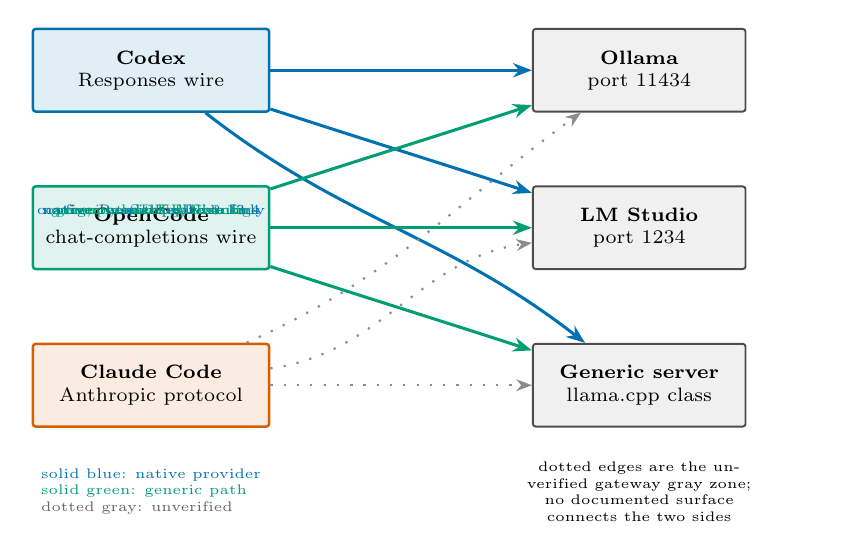
\begin{tikzpicture}[font=\scriptsize,
  agent/.style={draw=#1, line width=0.9pt, rounded corners=1pt, fill=#1!12,
    text=black, minimum width=3.0cm, minimum height=1.05cm, align=center},
  server/.style={draw=black!70, line width=0.7pt, rounded corners=1pt,
    fill=black!6, text=black, minimum width=2.7cm, minimum height=1.05cm,
    align=center},
  nat/.style={-{Stealth[length=2.4mm]}, line width=1.1pt, nativecol},
  gen/.style={-{Stealth[length=2.4mm]}, line width=1.1pt, genericcol},
  unv/.style={-{Stealth[length=2mm]}, line width=0.8pt, black!45, loosely dotted}]
% agents
\node[agent=nativecol] (cx) at (0, 2.0) {\textbf{Codex}\\ Responses wire};
\node[agent=genericcol] (oc) at (0, 0.0) {\textbf{OpenCode}\\ chat-completions wire};
\node[agent=unattcol] (cc) at (0,-2.0) {\textbf{Claude Code}\\ Anthropic protocol};
% servers
\node[server] (ol) at (6.2, 2.0) {\textbf{Ollama}\\ port 11434};
\node[server] (lm) at (6.2, 0.0) {\textbf{LM Studio}\\ port 1234};
\node[server] (gn) at (6.2,-2.0) {\textbf{Generic server}\\ llama.cpp class};
% Codex edges
\draw[nat] (cx) to[out=0, in=180] (ol)
  node[sloped, midway, above, font=\tiny, text=nativecol, pos=0.5] {native; version gate 0.13.4};
\draw[nat] (cx) to[out=-18, in=162] (lm)
  node[sloped, midway, above, font=\tiny, text=nativecol, pos=0.52] {native; model pull via lms};
\draw[nat] (cx) to[out=-38, in=142] (gn)
  node[sloped, midway, above, font=\tiny, text=nativecol, pos=0.58] {config; Responses wire only};
% OpenCode edges
\draw[gen] (oc) to[out=18, in=198] (ol)
  node[sloped, midway, above, font=\tiny, text=genericcol, pos=0.48] {generic; baseURL config};
\draw[gen] (oc) to[out=0, in=180] (lm)
  node[sloped, midway, above, font=\tiny, text=genericcol, pos=0.5] {generic; catalog fixture};
\draw[gen] (oc) to[out=-18, in=162] (gn)
  node[sloped, midway, above, font=\tiny, text=genericcol, pos=0.52] {compat-SDK fallback};
% Claude Code edges: unverified gray zone
\draw[unv] (cc) to[out=24, in=216] (ol);
\draw[unv] (cc) to[out=8, in=188] (lm);
\draw[unv] (cc) to[out=0, in=180] (gn);
\node[align=center, font=\tiny, text width=4.6cm] at (6.2,-3.35)
  {dotted edges are the unverified gateway gray zone;\\ no documented surface connects the two sides};
\node[align=left, font=\tiny] at (0,-3.35)
  {\textcolor{nativecol}{solid blue: native provider}\\
   \textcolor{genericcol}{solid green: generic path}\\
   \textcolor{black!60}{dotted gray: unverified}};
\end{tikzpicture}
\caption{Support as a graph. Solid arrows are attested paths with their
tier; dotted arrows mark the \ccc{} gray zone where no source attests the
connection. Values match Table~\ref{tab:matrix}.}
\label{fig:support}
\end{figure}

Read together, the matrix, the caveats, and Figure~\ref{fig:support}
support one directional claim:
compatibility with open models is decided by the wire protocol an agent
commits to. \codex{} committed to Responses and built native plumbing
for two local servers, accepting the patch-tool loss and betting on
server-side adoption. \occ{} committed to nothing and accepts anything
chat-completions-shaped, accepting that its accounting defaults misbehave
around zero limits. \ccc{} commits to Anthropic's stack and leaves the
rest to whatever the user can route through a gateway, unattested.

\section{Synthesis: one architecture, three cultures, one stress test}
\label{sec:synthesis}

\subsection{Convergence and divergence in harness architecture}
\label{sec:convergence}

The evidence points to one shared architecture with three engineering
cultures.

\paragraph{Convergence.} (1) All three implement the abstract
prompt-sample-execute-continue loop and all three encode an explicit
anti-loop defense (rejection taxonomy; identical-call tripwire; stop-hook
cap). (2) The patch format is converging across vendors: \occ{} ports the
\codex{} \path{apply_patch} format verbatim in type names and selects it
for OpenAI model IDs, evidence of cross-harness borrowing at the protocol
level. (3) Extension vocabularies are converging on the \ccc{} design:
\codex{} exports \path{CLAUDE_PLUGIN_ROOT} compatibility variables and
discovers \path{.claude-plugin} manifests, and \occ{} reads \path{.claude}
skill layouts and CLAUDE.md files as fallbacks. (4) MCP is the shared
external-tool boundary in all three, with \codex{} exposing itself as an
MCP server (\path{codex} and \path{codex-reply} tools), and both open
systems naming MCP tools by server-prefixed identifiers. (5) All three
gate dangerous defaults behind enterprise layers (managed settings,
\path{requirements.toml}, MDM plists).

\paragraph{Genuine divergence.} (1) Control flow: task state machine
against persistence-driven loop against an undisclosed closed loop.
(2) Tool registration: conditional per-turn registration against a fixed
array against a partly documented inventory. (3) Safety substrate: OS
sandbox plus rule engine against in-process rules only against a Bash-scoped
OS sandbox plus permission layer. (4) Compaction triggers: fractional
window against reserved buffer against undisclosed. (5) State: JSONL-first
with a repairable SQL mirror against SQL-event-first with shadow-git file
history against undisclosed. (6) Interface philosophy: one protocol for
every frontend against a local HTTP server consumed by every frontend
against documented-only surfaces. Naming differences (hooks, skills,
agents/subagents, plugins) overlay these structural differences rather than
masking them.

\subsection{Part II is Part I's configuration dimension under stress}
\label{sec:crossreading}

The compatibility findings do not add a ninth machinery dimension; they
sharpen the configuration-and-providers dimension of
Section~\ref{sec:config}, and each system's open-model behavior is what
Part I's architecture predicts.

\codex{}'s reserved provider IDs and Responses-only wire become, under
open models, two native local-server entries with a version gate and a
hard refusal of everything else; its protocol-first interface culture
(Section~\ref{sec:state}) is the same instinct as pinning the Responses
wire end to end. \occ{}'s widest-in-the-study provider layer becomes the
widest open-model acceptance, and its permissive configuration culture
reappears as permissive accounting defaults: zero limits silently disable
compaction or balloon output requests. \ccc{}'s closed loader stays
closed for model wiring, and Part I's advisory-against-enforcement split
reappears as documented Anthropic-cloud enforcement plus pass-through
variables whose wire behavior is unattested
(Sections~\ref{sec:compatcodex} to~\ref{sec:compatccc}).

One thread runs through both parts without branching: the patch tool.
\occ{} selects between \path{apply_patch} and \path{edit}/\path{write} by
model ID (Section~\ref{sec:tools}); for open models that gate resolves to
the edit paths in \occ{} and to no patch tool at all under \codex{}'s
fallback metadata (Sections~\ref{sec:compatcodex},~\ref{sec:compatopencode}).
The compaction constants of Section~\ref{sec:compaction} compose with the
Part II findings the same way: they only govern once the accounting
inputs are corrected by hand, since \codex{} assumes a 272{,}000-token
window on catalog misses, \occ{} disables auto-compaction at a zero
context limit, and \ccc{} can defer enforcement to a server error a
gateway may rewrite.

\subsection{Design lessons}
\label{sec:lessons}

Seven takeaways for a reader building or choosing a harness, each
supported by a section above. (1) Anti-loop machinery is not optional:
the repetition failure modes ReAct measured reappear in production form,
and every system has an explicit answer, a typed rejection taxonomy, an
identical-call tripwire, or a stop-hook cap
(Section~\ref{sec:turnloop}). (2) The edit protocol is worth engineering
money: a grammar-parsed patch format and a nine-stage fuzzy replacer are
two responses to the same measured fragility, and the patch format is
already being ported across vendors (Section~\ref{sec:tools}).
(3) The kind of compaction trigger a system chooses, a fraction of the
window or a reserved headroom, reveals its accounting philosophy, and
tool output is where the bloat budget should go
(Section~\ref{sec:compaction}). (4) Recoverability is a safety
mechanism, not a feature: per-step snapshots with revert allow a
permissive default policy (Sections~\ref{sec:safety},~\ref{sec:state}).
(5) A good documented contract can substitute for a plugin API: \ccc{}'s
stop hook carries an unbounded autonomous loop with no core changes
(Section~\ref{sec:extensibility}). (6) The wire protocol an agent commits
to decides its open-model reach; every commitment has a matching price,
paid in a different currency (Sections~\ref{sec:servers},~\ref{sec:matrix}).
(7) For open models, fill in the accounting before the first session:
limits, patch-tool expectations, and window enforcement defaults are the
three places the studied harnesses misbehave silently
(Section~\ref{sec:matrix}).

\section{Related Work}
\label{sec:related}

Organized by comparison dimension.

\paragraph{Loop control and tool protocols.} ReAct established interleaved
reasoning and acting as the canonical agent loop and measured its
hallucination and repetition failure modes~\citep{yao2023react}; Toolformer
learned the tool-call emission protocol and constrained decoding to avoid
tool-call loops~\citep{schick2023toolformer}. The studied harnesses move
both concerns from prompting into machinery: typed rejection taxonomies,
identical-call tripwires, and stop-hook caps are engineering versions of
the same defenses.

\paragraph{Agent-computer interfaces and editing.} SWE-agent showed
interface design moves coding-agent performance: a guarded edit command and
lint gating each contributed measurable gains, while an iterative search
interface hurt~\citep{yang2024sweagent}. Our tool-surface findings extend
this from benchmark scaffolds to shipping products: all three systems
converge on structured edit protocols (grammar-parsed patches, staged
fuzzy replacers, documented edit tools), consistent with SWE-agent's
evidence that free-form shell editing is the failure-prone baseline.

\paragraph{Safety for tool-using agents.} ReAct's ethics statement limited
its action space to benign websites precisely because acting on real
environments is dangerous~\citep{yao2023react}; SWE-agent used Docker
containers with no permission model~\citep{yang2024sweagent}. The three
harnesses represent the next stage: per-command policy engines with OS
sandboxing, in-process permission rulesets, and layered permission-plus-
sandbox models with documented protected paths. Within our scope, none of
the three pinned sources cross-references the academic literature in its
policy design; the connection above is ours, grounded in the shared
failure patterns each mechanism addresses.

\paragraph{Distinction from nearest work.} The nearest verifiable work is
the SWE-agent interface study, which ablates interface choices for one
external agent on one benchmark~\citep{yang2024sweagent}. This study
instead traces three closed-loop products at the implementation level,
covers eight machinery dimensions plus an open-model compatibility trace
against three reference servers, and treats a closed-source system with a
documentation-tier protocol. Its bounds are correspondingly different:
no behavior was executed, and every claim is version-pinned. For Part II,
the compatibility question is ordinarily answered by community test
reports; here it is answered by source traces, which trade runtime
coverage for pinning and anchorability. The community router around
\ccc{} sits in the nearest-work neighborhood as an existence proof that
users route around the closed loader, not as
evidence~\citep{claudeCodeRouterContext}.

\paragraph{Third-party teardowns.} Three teardowns of \ccc{} were reviewed
and held to contextual use only: an intercepted-log teardown reporting
system-prompt and tool-token sizes and small-model routing
(minusXTeardown~\citep{minusXTeardown}), a binary-analysis catalog of
feature flags, telemetry events, and tools~\citep{tenguDecoded}, and a
trace-based breakdown of extension layers whose memory-delivery shape is
cross-verified by official documentation~\citep{agiflowInternals}. None
carries a comparison cell; their assertions are unverified against any
primary source.

\section{Limitations}
\label{sec:limitations}

\paragraph{Version bounds.} Every code claim is bounded to the three pinned
commits; every documentation claim to snapshots fetched 2026-08-20 from
sites that are not version-pinned and can drift. Nothing generalizes to
newer releases, and the \occ{} pin is the \texttt{dev} branch of the
rewrite, not a released version.

\paragraph{No behavior was measured.} The study is static by design. No
agent was run, no API was called, no server served, and no code from the
pinned repositories was executed. Statements about defaults and triggers
describe code paths and documentation contracts, not observed runtime
behavior. The validation runs re-check anchors but are smoke-test
plumbing, not evidence about the systems. In Part II, the practical
consequence is that server acceptance of agent request fields (tools
JSON, parallel calls, reasoning fields) is the single largest uncheckable
cell~\citep{codexRepo,lmstudioApiDocs}.

\paragraph{Closed core.} The \ccc{} turn loop, tool registry, compaction
thresholds, session storage, permission-enforcement internals, sandbox
mechanisms, and model loader are not established by this study; all are
documented contracts or surface attestations. The pinned documentation
set also lacks the compaction-survival page referenced by the memory
docs, so the survival rules beyond root CLAUDE.md are incomplete, and the
wire shape of \ccc{} gateway traffic is nowhere attested, which leaves
both the pass-through mechanism and any Anthropic-compatible-server
hypothesis uncheckable (Section~\ref{sec:compatccc}). Documentation
describes intended behavior, not necessarily shipped behavior on every
platform.

\paragraph{Teardown and router tier.} Third-party teardowns and the
community router are unverified claims about captures, binaries, and
gateways this study cannot inspect; they appear only as hedged context.
One blog assertion (the memory-delivery shape) is corroborated by
official documentation, and only that overlap is treated as reinforced.

\paragraph{Server snapshot coverage.} The Ollama snapshot is the 2024
compatibility post, which predates the version \codex{} requires;
current Ollama behavior beyond that gate is not covered. LM Studio
snapshots came from its documentation repository because the live site
was unreachable from the study environment, so drift from the shipped
application is unassessed. The llama.cpp snapshot is master at fetch
time, unversioned. vLLM's compatible-server documentation moved and could
not be re-located within budget, so the generic bar is carried by
llama.cpp and LM Studio alone.

\paragraph{Catalog state and fallback metadata.} \occ{}'s live model
catalog is runtime state; only the pinned test fixture is inspectable, so
claims about catalog contents are fixture-scoped. \codex{}'s patch-tool
loss and the 272{,}000-token accounting rest on catalog misses resolving
to a fallback description; whether that fallback survives at runtime
depends on the models-catalog refresh decoding against a plain
\path{/v1/models} listing, which expects the rich catalog schema and is
not exercised against a local server in the pinned
tree~\citep{codexRepo,opencodeRepo}. Two compaction implementations
coexist in the pinned \occ{} tree, and which one serves the default run
was not traced; the reserve figures are attributed to the v1 overflow
path~\citep{opencodeRepo}.

\paragraph{Open cells.} Where no pinned source states a value, the
sections above say so explicitly: \ccc{} compaction thresholds, loop
implementation, full tool registry, provider plumbing, and gateway wire
shape; \occ{} permission merge precedence, runtime enforcement of several
schema defaults, and compaction path selection; \codex{} remote
model-catalog and enterprise cloud-bundle contents, which are server-side
state. These are evidence gaps, not findings of absence, except where
stated (for example, the absence of an OS sandbox in the pinned \occ{}
tree and the absence of any open-model mention in the \ccc{} snapshots
are searched-scope results).

\section{Conclusion}

Three production harnesses implement the same abstract coding-agent loop
and diverge at every level below it. \codex{} builds a typed state machine
over abortable tasks, wraps shell access in an OS sandbox plus a rule
engine, persists threads as inspectable JSONL with an exact replay path,
and gives open models the deepest first-class support via native
Responses-API providers, at the cost of the patch tool on those defaults.
\occ{} builds a persistence-driven loop over a fixed tool array, keeps all
policy in-process, invests its safety budget in recoverable state, and
gives open models the broadest support at the cost of accounting defaults
that misbehave around zero limits. \ccc{} presents a documentation-defined
contract over a closed core: a wide hook lifecycle, a two-layer
permission model with a Bash-only OS sandbox, an extension surface whose
stop-hook escape hatches already implement autonomous loops outside the
core, and no documented open-model path at all. Read as a catalog, this
report describes three systems twice: once as harnesses, once as
platforms for open-weight models. Read as design material, it is eight
questions carrying two concrete answers and one boundary each, plus one
variable, the wire protocol, that predicts where each system lands on the
compatibility matrix. For a reader choosing today: the abstraction is
settled (loop, tools, compaction, permissions, extensions) while the
engineering culture is not, and if open models are in scope, point
\occ{} at anything OpenAI-compatible after setting limits by hand, run
\codex{} against Ollama 0.13.4 or newer or LM Studio with gpt-oss models,
and treat \ccc{} with local models as a community-project problem until
the vendor says otherwise. All conclusions are bounded to the pinned
commits and documentation snapshots named in Section~\ref{sec:methods}.

\bibliographystyle{plainnat}
\bibliography{refs}

\end{document}
